%\addcontentsline{toc}{chapter}{Development Process}
\chapter{Design}
This design chapter aims to outline the design ideas and thought processes of the initial planning stage of the project. 

\section {The LED Profile Objects}
The LED profile object was the main container of information in the code that stored all of the visual data that was printed to the LEDs. It was essential to have two versions of the LED profile. This was because the standard and addressable LEDs needed to store different content. The initial plan was to have the following elements stored in the LED profile object:
\begin{itemize}
\item Profile Name - A modifiable string with no limitations. Initially, this was a base name that the user was directed to change at the beginning of its creation to identify the profile e.g. Fireplace, welding lights, flickering bulb etc. 

\item Trigger - This element would come in the form of a String which would be restricted to being words which relate to the different types of triggers talked about in 1.2 Analysis e.g. trigger = "Time"

\item Trigger parameters - Preceding the trigger were all of the possible different parameter variables e.g. the start and end time, temperature threshold etc . These supplemented the trigger. They identified the specific environmental conditions that activated the profile and commenced specific activities within the diorama or model. 

\item LED Brightness array - This was the main array for the standard LED profile. This was an unrestricted array containing all the brightness values available for the main lighting loop to access when activating the LEDs.

\item Addressable LED colour array - The addressable LED profiles used a similar container to the brightness array from the standard LED profiles to display the final colour. The brightness array was replaced by three different arrays corresponding to red, green and blue. For example, When the values from the first element in each array were inputted into the display function of the LED, the LED would display the appropriate RGB colour. This was repeated until the desired colour sequence was achieved.

\item LED duration - The LED duration is an integer that defined the number of iterations needed to pass before the next brightness is displayed. 
\end{itemize}

\section{The LED Object}
While the LED profile object (outlined above) contains all of the information on how the LED is displayed, the LED object stores all of the information about the LED itself. These are the elements that would be stored in the LED object:
\begin{itemize}
\item LED channel - This is the value that was referenced each time we wanted to print a new brightness to the LED.

\item PinOut - An integer to represent which pin was attached to the LED.

\item The LED profile - This was how the two objects were connected to each other. The LED object contained a profile object which was the profile assigned to that LED.
\end{itemize}

\section{Code Design}
One of the biggest design concepts implemented into the coding element of the project was the idea of flexibility. Where there was greater flexibility in the type of profile the user developed, this created a better range of lighting sequences. In turn, this produced a more realistic lighting effect for the diorama/model scenario. 

Flexibility within the project were a fundamental part of the design. Customisation of the project enabled the user to fully engage with the final design of the lighting for the diorama.  This customisation allowed the user to vary the length of the LED profile and how long the LED profile played for. This was achieved by the user being able to customise the following:

\subsection {Duration of the iteration}
By adding a customisable interaction size to the main code loop of the program gave the user more flexibility in the final display performed by the LEDs. For example, if the iteration size were smaller, this allowed the user to have a smoother transition between colours e.g. the changing colour of the sky. If the iteration size was larger, it allowed for displays such as red flashing lights at a train crossing. This time scale had its limitations however, depending on how long it took for the code to traverse through the main code loop. 

\subsection {Number of iterations before next colour/ brightness display}
This allowed the user to have multiple LEDs transitioning at different time scales. For instance, this allowed both of the LED functions talked about in the previous points (fast gradual transitions and slow dramatic transitions) to be displayed at the same time. 

\subsection {Unrestricted length of profile array(s)} 
By having an unrestricted profile length this allowed the user to have any number of brightness/colours before the end of the array. However, this restricted how often the profile could be activated by its trigger and was stuck completing the entire sequence before it was able to be played again e.g. The lighting sequence cannot be stopped midway through the display.

\subsection{The design of the main lighting loop}
If the main lighting loop , which is what sets the LEDs to their specified colour/brightness, was coded in the correct way, it allowed for any number of LEDs to be played at any one time. However, the more LEDs active at one time limited how fast the iteration could be completed.

\section{Website Design}
The main aspect that needed to be considered with the website design was its ease of use. As some of the clientele for the program may not be tech-savvy or experienced in coding, it was imperative that the program webpage was clearly laid out and the profiles were easily modified. The overall design chosen is loosely based on the code blocks from a programming learning tool called Scratch.

\begin{figure}[h]
\begin{subfigure}{0.5\textwidth}
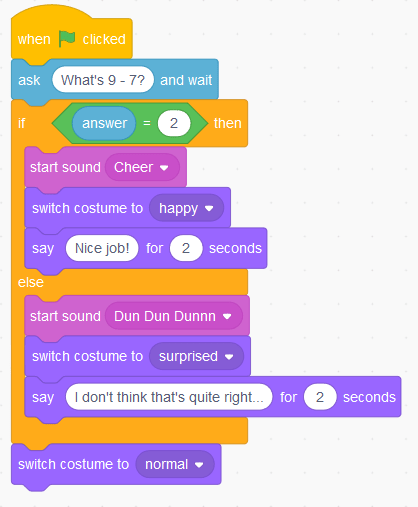
\includegraphics[width=0.9\linewidth, height=6cm]{Scratch}
\caption{scratch example}
\end{subfigure}
\begin{subfigure}{0.5\textwidth}
\rotatebox{90}{
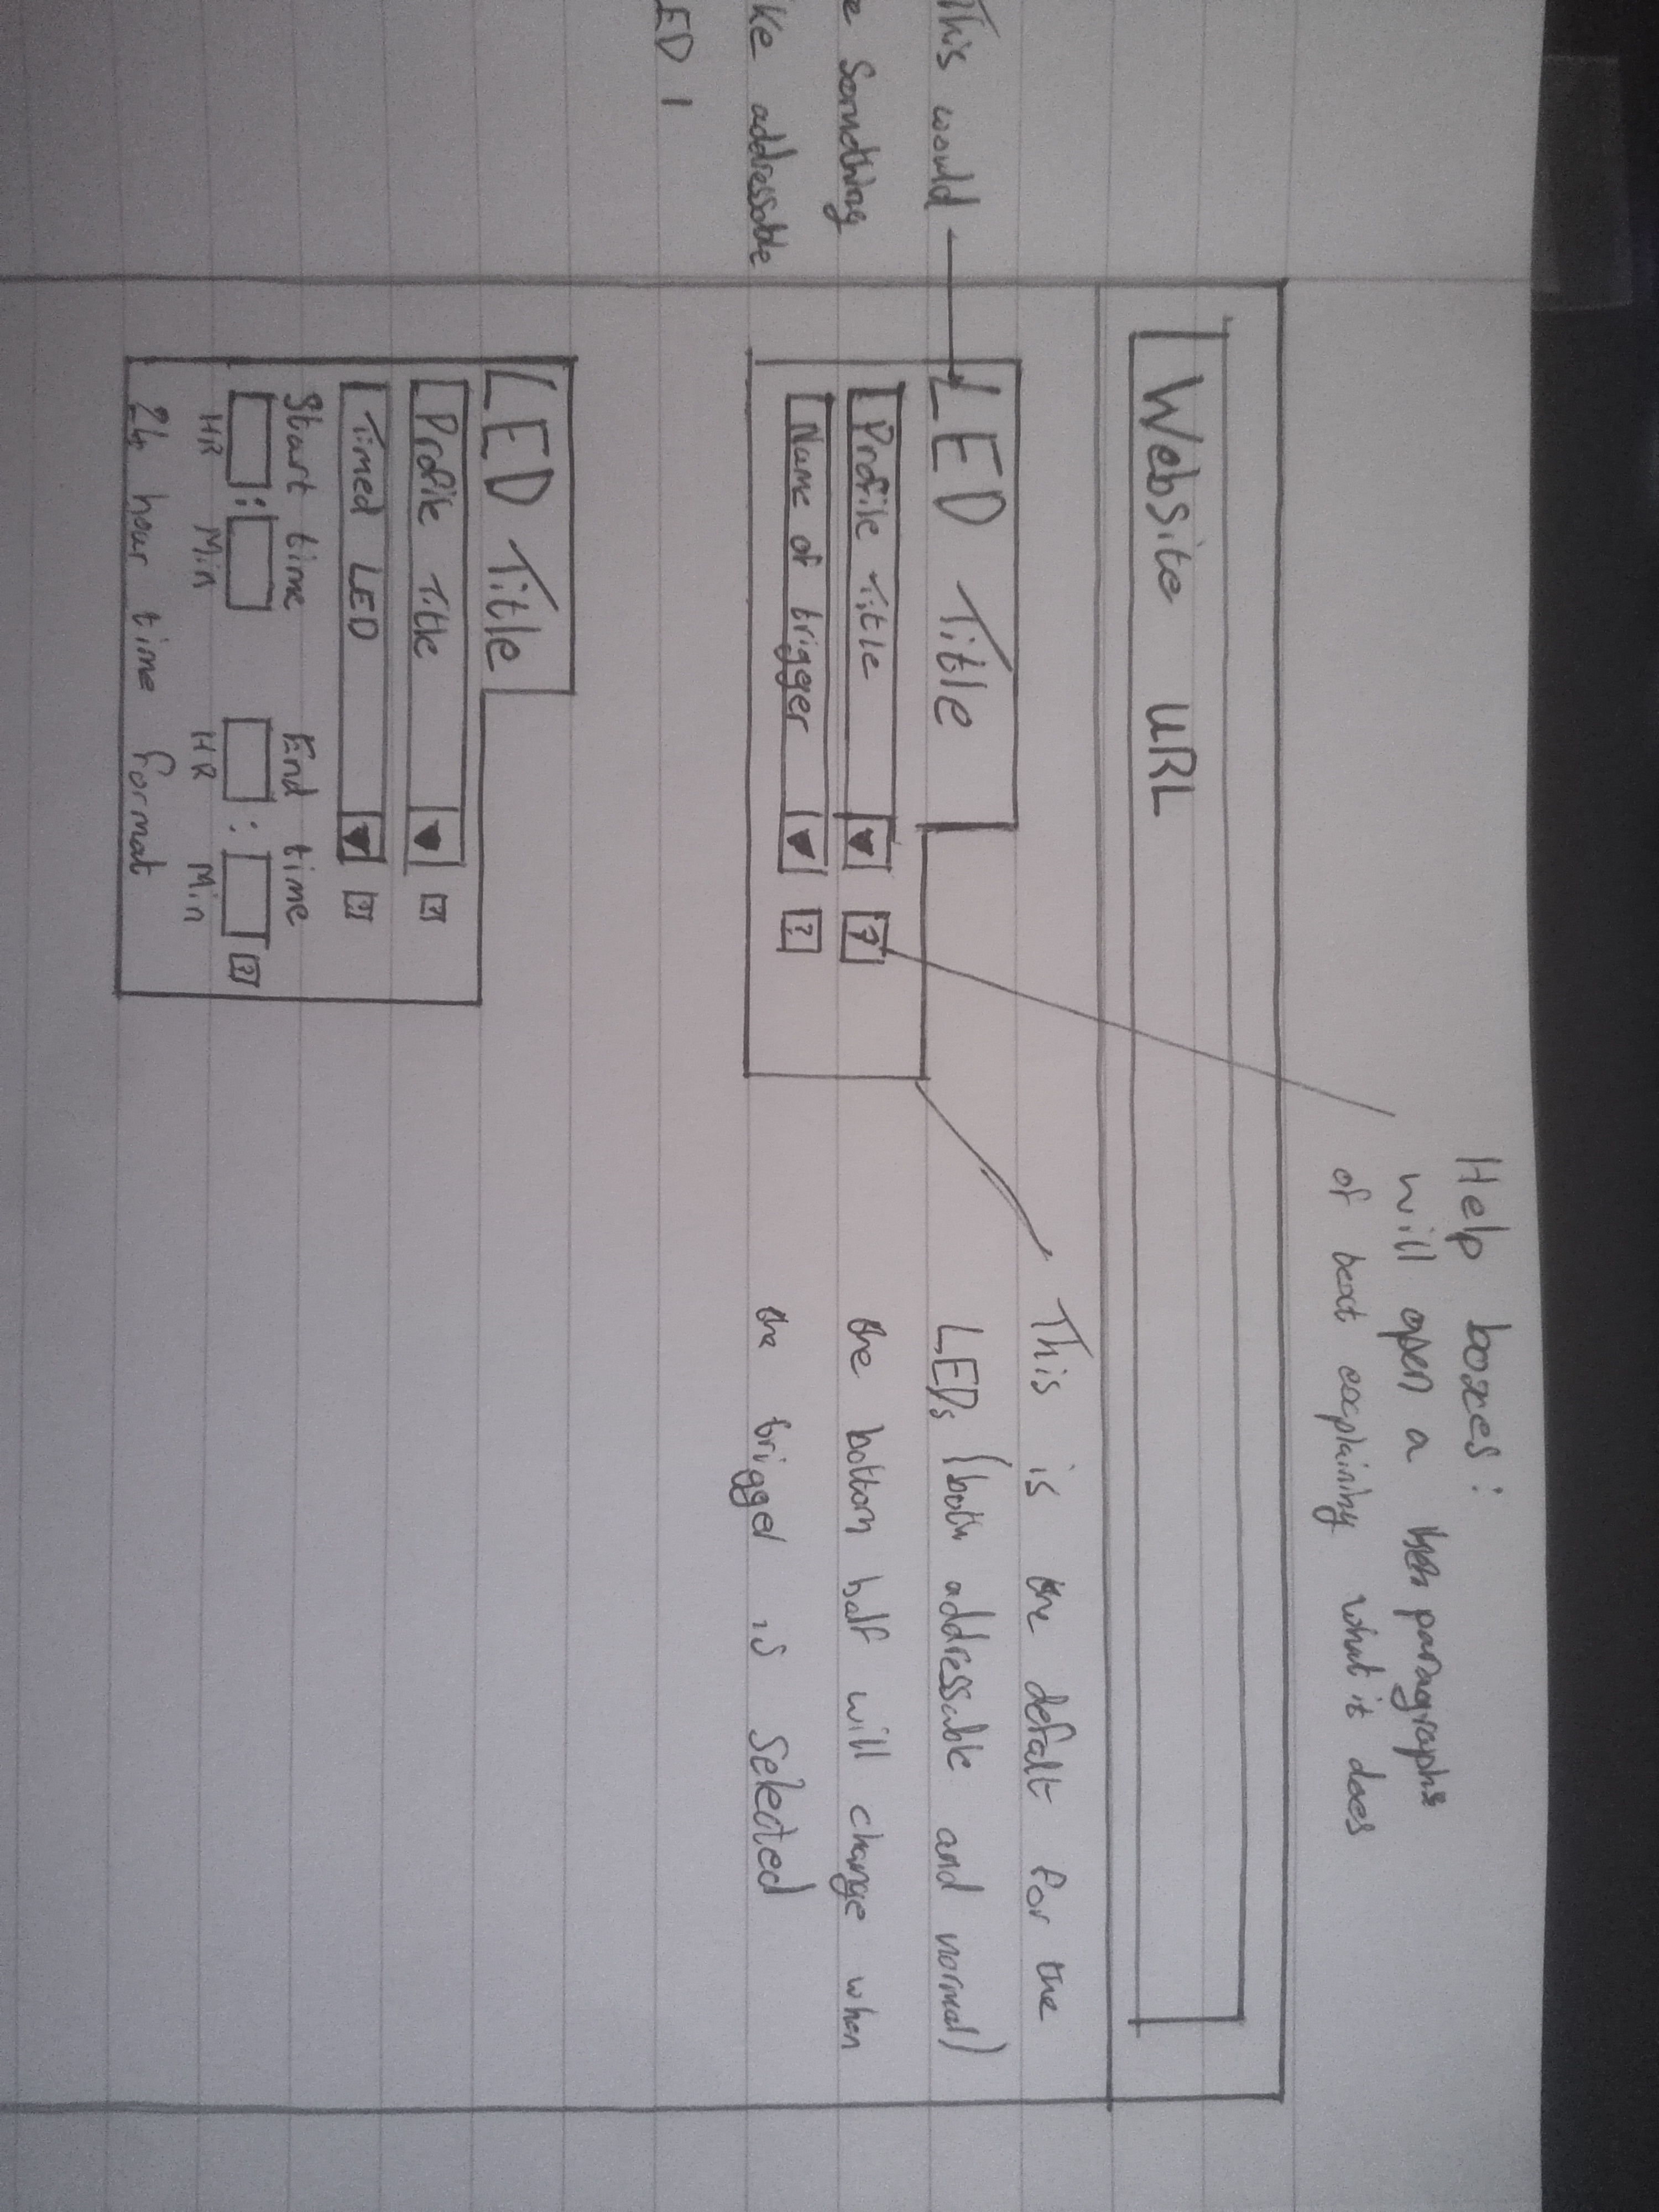
\includegraphics[width=0.8\linewidth, height=7cm]{UIDesign}}
\caption{Drawing of intended UI Design}
\end{subfigure}

\caption{Comparison Between Scratch and My UI Design}
\end{figure}

It was decided the use of code blocks, which is a similar concept on which Scratch is based on \cite{Scratch}, would make it easier for the user to understand what they were currently working on. When a trigger was chosen for the LED, additional input options were added to choose the parameters of the trigger. The additional input options depended on what trigger was chosen. For instance, if the time trigger were selected, four additional boxes appeared so that the user could enter the start and end time in hours and minutes. However, if the temperature trigger was selected, only one box would appear along with an additional drop-down box. This enabled the user to enter the threshold in which the temperature would trigger and then whether they wanted it triggering above or below this threshold. Also, to make it easier for the user to understand the expected input, there was a help box that the user could access for a description and a explanation.  This showed the user a paragraph of text explaining what they were choosing and what the expected input would look like.
